
\subsection{MATLAB}
\label{MATLABPID}

Príklad na ukážku fungovania PID regulátora bol taktiež vytvorený v prostredí MATLAB a simulink. V prípade MATLABU využívame, na výpočet akčného zásahu, knižnicu PID.m, ktorá bola taktiež vytvorená v rámci programu AutomationShield. Na nastavenie parametrov PID slúži príkaz \code{PID.setParameters(Kp, Ti, Td, Ts)}. 

Na vzorkovanie využívame funkcie \verb|TIC a TOC |, ktoré merajú prejdený čas. Funkcia TIC zaznamenáva aktuálny čas a funkcia TOC používa zaznamenanú hodnotu na výpočet uplynulého času. Ak je splnená podmienka \code{if (toc>=Ts*k)}, povolí sa posun na nasledujúcu vzorku, pričom premenná \verb*|k|, udáva počet vykonaných vzoriek. Dáta sú postupne zapisované do poľa \code{ PIDresponse(k,:)=[r y u]}, a toto pole je vykresľované pomocou funkcie \code{plotLive(PIDresponse(k,:))}. Na konci sú všetky dáta uložené, a teda sú prístupné aj po ukončený programu. Kompletný zdrojový kód sa nachádza v prílohe na strane \pageref{AeroShieldPID.m}.

Regulácia PID v prostredí MATLAB potrebuje pre svoje fungovanie pomerne vysoký výpočtový výkon počítača, pretože výpočty prebiehajú na zariadení s ktorým je Arduino prepojené. Na zariadení\cite{Notebook} v ktorom boli písané všetky didaktické príklady dosahujeme rýchlosť maximálne piatich vzoriek za sekundu tj. Ts=0.2s. Pri pomalšom vzorkovaní musíme spomaliť aj rýchlosť reakcie PID regulátora (napr. znížením proporcionálnej zložky). Výpočtová náročnosť sa dá znížiť, zamedzením vykresľovania grafu, alebo odstránením možnosti ukladania zaznamenaných dát. 

\begin{figure}[!tbh]
	\centering
	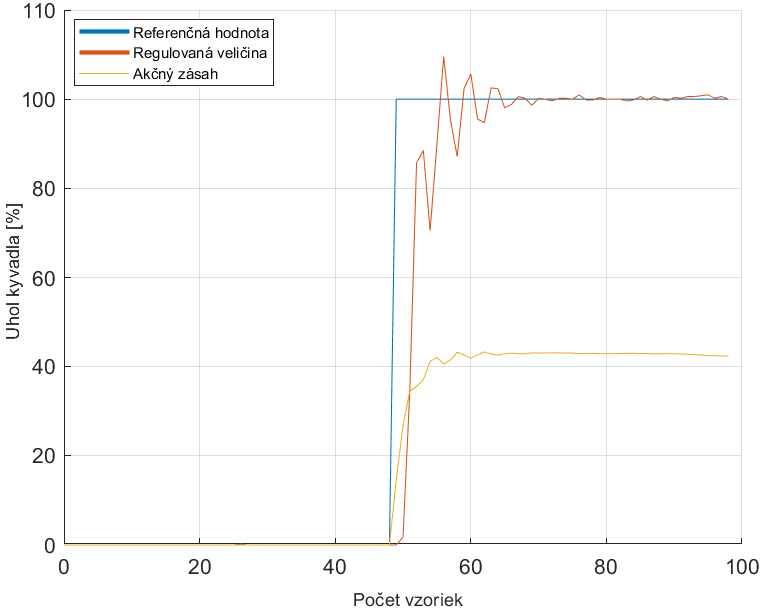
\includegraphics[width=90mm]{obr/jednotkovyskoskMAt.png}
	\caption{Reakcia systému na jednotkový skok referenčnej hodnoty.}\label{OBRAZOK 2.6.1}
\end{figure}

\subsubsection{Výstupy}

Všetky výstupy z príkladu \ref{MATLABPID}, majú priamu funkciu vykresľovania grafov spolu s legendou výstupov. Tieto grafy majú taktiež definovaný rozsah zobrazovaných hodnôt na oboch osiach, ako aj pomenovania týchto osí. Na obr.\ref{OBRAZOK 2.6.1} vidíme reakciu systému na jednotkový skok. Obrázok \ref{OBRAZOK 2.6.2} zobrazuje automatickú trajektóriu referenčnej hodnoty a obr.\ref{OBRAZOK 2.6.3} trajektóriu manuálnu. 

Pri manuálnej trajektórii bola trikrát vnesená veľká chyba a to pomocou úderu do kyvadla. Ako je vidieť z grafu \ref{OBRAZOK 2.6.3}, ustálenie systému prebieha oveľa pomalšie ako v príklade \ref{Arduino IDE PID}. Oscilácia je pomerne vysoká a pretrváva po dobu cca 35 vzoriek, čo predstavuje približne 7 sekúnd. Táto skutočnosť je spôsobená pomalšou reakciou PID regulátora, na veľkú regulačnú odchýlku. Dlhší čas potrebný na ustálenie kyvadla je spôsobený predovšetkým pomalším vzorkovaním.  
\vspace{6cm}

\begin{figure}[!tbh]
	\centering
	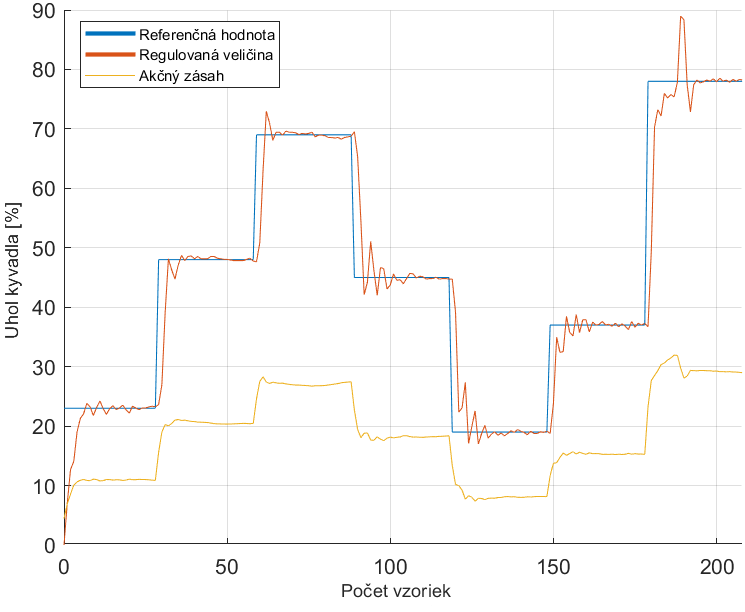
\includegraphics[width=125mm]{obr/PIDautomaMat.png}
	\caption{Automatická trajektória.}\label{OBRAZOK 2.6.2}
\end{figure}
\begin{figure}[!tbh]
	\centering
	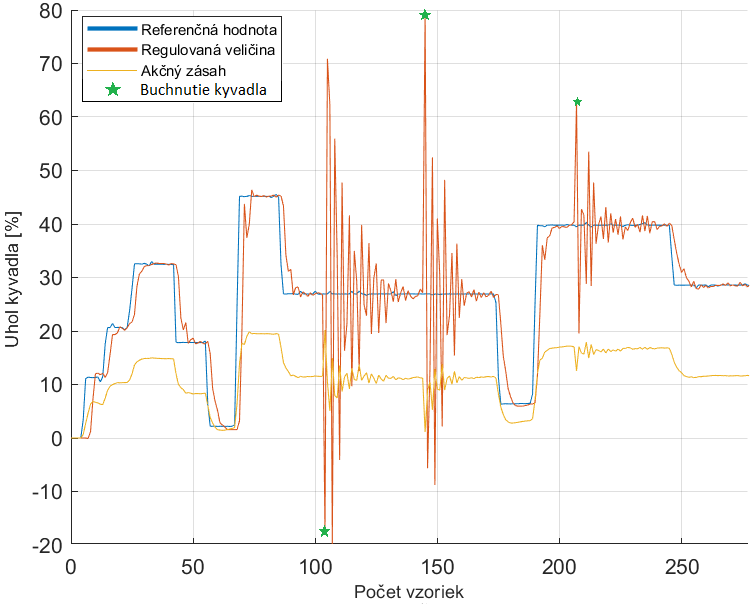
\includegraphics[width=125mm]{obr/pidmanualbuchh.png}
	\caption{Manuálna trajektória.}\label{OBRAZOK 2.6.3}
\end{figure}

\newpage 
\subsection{Simulink}

Vzhľadovo pôsobí príklad PID riadenia v API Simulink jednoducho a elegantne. Predpripravené bloky z knižnice AeroLibrary stačí v príklade pospájať podľa potreby a následne zvoliť vhodné parametre v maskách blokov. Prepájanie blokov slúži na spájanie vstupov s výstupmi, alebo na matematické operácie s premennými. Regulovanú sústavu v tomto príklade predstavuje blok \verb|AeroShield|, do ktorého vstupuje z bloku \verb|Reference read| percentuálna hodnota referenčnej trajektórie. Z bloku \verb|AeroShield| máme ako výstup uhol kyvadla, ktorý využívame na výpočet regulačnej odchýlky.  

Blok \verb|Discrete PID Controller| predstavuje riadiaci systém PID regulátora. Hodnoty jednotlivých zložiek regulátora sú: P=0.011, I=200, D=8. Matematická reprezentácia výpočtového algoritmu ideálneho PID regulátora, je v tvare rov.\ref{PIDSimulink}:

\begin{equation}\label{PIDSimulink}
	P\left(1+I*T_s\dfrac{1}{z-1}+D*\dfrac{1}{T_s}\dfrac{z-1}{z}\right)
\end{equation}


\begin{figure}[!tbh]
	\centering
	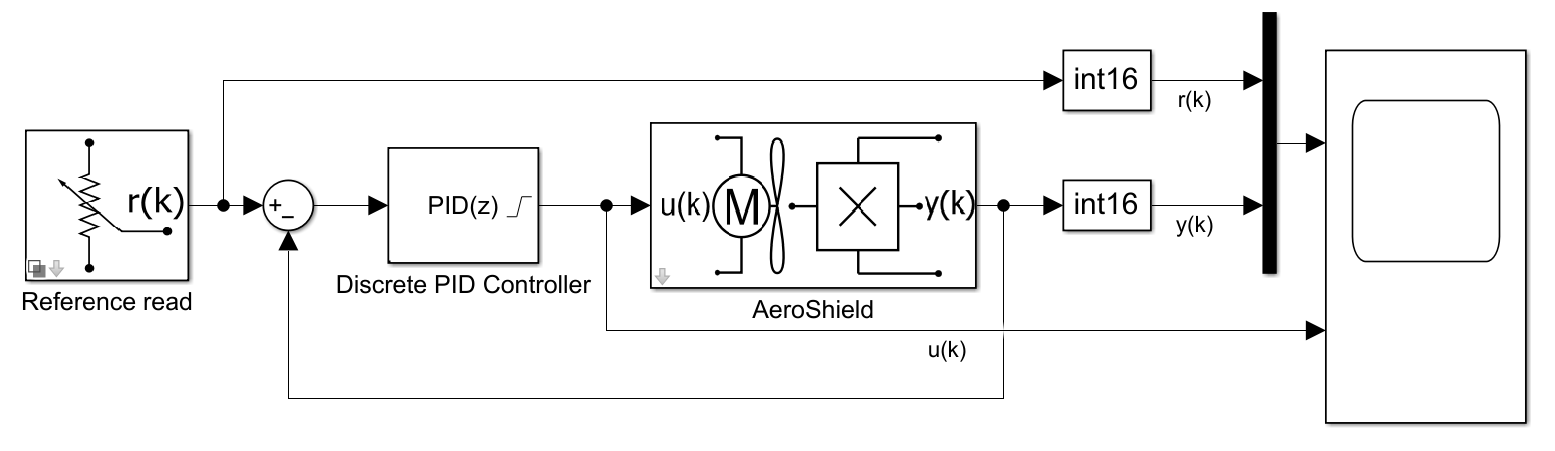
\includegraphics[width=125mm]{obr/SimulinkPID.png}
	\caption{Ukážka riadenia systému pomocou PID regulátora v API Simulink.}\label{OBRAZOK 2.6.10}
\end{figure}

\subsubsection{Výstupy}

\begin{figure}[!tbh]
	\centering
	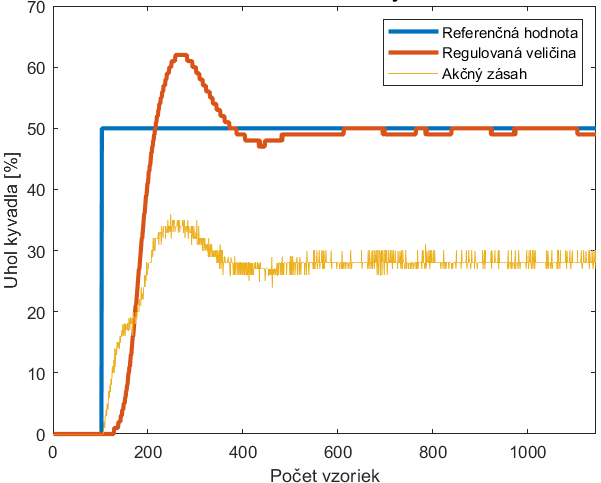
\includegraphics[width=100mm]{obr/SimSkok.png}
	\caption{Reakcia systému na skokovú zmenu referenčnej hodnoty.}\label{OBRAZOK 2.6.11}
\end{figure}

\begin{figure}[!tbh]
	\centering
	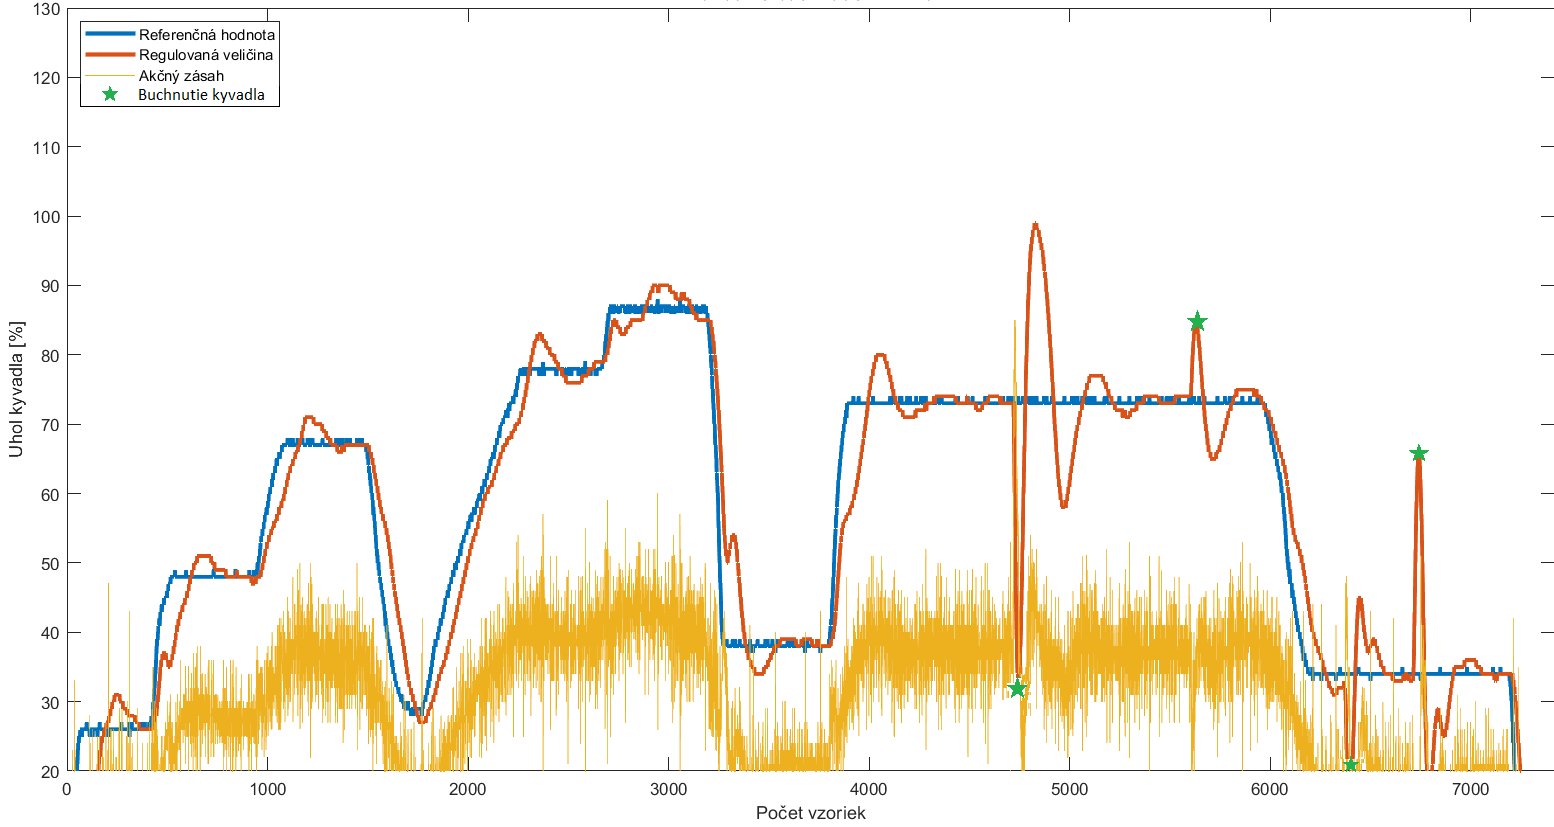
\includegraphics[width=125mm]{obr/SimulinkManualBuch.png}
	\caption{Manuálna trajektória.}\label{OBRAZOK 2.6.12}
\end{figure}